\documentclass[
    xcolor={svgnames,dvipsnames},
    hyperref={colorlinks, citecolor=DeepPink4, linkcolor=DarkRed, urlcolor=DarkBlue}
    ]{beamer}  % for hardcopy add 'trans'

\mode<presentation>
{
  \usetheme{Singapore}
  % or ...
  \setbeamercovered{transparent}
  % or whatever (possibly just delete it)
}



\addtobeamertemplate{navigation symbols}{}{%
    \usebeamerfont{footline}%
    \usebeamercolor[fg]{footline}%
    \hspace{1em}%
    \insertframenumber/\inserttotalframenumber
}



\usepackage{fontspec} 
%\usepackage[xcharter]{newtxmath}
%\setmainfont{XCharter}
\usepackage{unicode-math}
%\setmathfont{XCharter-Math.otf}
\setmonofont{DejaVu Sans Mono}[Scale=MatchLowercase] % provides unicode characters 

\usepackage{tikz}
\usetikzlibrary{shadows, trees, shapes.geometric, matrix, shapes, arrows.meta, positioning, fit, backgrounds, calc}

% \usetikzlibrary{matrix, arrows.meta, positioning, calc, backgrounds}

% for tikz
\usepackage{pgfplots}
\usepgfplotslibrary{fillbetween}
\pgfplotsset{compat=1.16}

\usepackage{varwidth}
\usepackage{minted}
\usemintedstyle{friendly}
\setminted[python]{
  fontsize=\small,
  baselinestretch=1.2,
  bgcolor=codebg,
  linenos=false,
  breaklines=true,
  frame=none
}
\setminted[matlab]{
  fontsize=\small,
  baselinestretch=1.2,
  bgcolor=codebg,
  linenos=false,
  breaklines=true,
  frame=none
}
\setminted[julia]{
  fontsize=\small,
  baselinestretch=1.2,
  bgcolor=codebg,
  linenos=false,
  breaklines=true,
  frame=none
}
%\setminted{mathescape, frame=lines, framesep=3mm}
%\newminted{python}{}
%\newminted{c}{mathescape,frame=lines,framesep=4mm,bgcolor=bg}
%\newminted{java}{mathescape,frame=lines,framesep=4mm,bgcolor=bg}
%\newminted{julia}{mathescape,frame=lines,framesep=4mm,bgcolor=bg}
%\newminted{ipython}{mathescape,frame=lines,framesep=4mm,bgcolor=bg}

\usepackage{graphicx}
\usepackage{amsmath, amssymb, amsthm}
\usepackage{bbm}
\usepackage{mathrsfs}
\usepackage{xcolor}
\usepackage{fancyvrb}


% Quotes at start of chapters / sections
\usepackage{epigraph}  
\renewcommand{\epigraphwidth}{6in}

%% Fonts

%\usepackage[T1]{fontenc}
\usepackage{mathpazo}
%\usepackage{fontspec}
%\defaultfontfeatures{Ligatures=TeX}
%\setsansfont[Scale=MatchLowercase]{DejaVu Sans}
%\setmonofont[Scale=MatchLowercase]{DejaVu Sans Mono}
%\setmathfont{Asana Math}
%\setmainfont{Optima}
%\setmathrm{Optima}
%\setboldmathrm[BoldFont={Optima ExtraBlack}]{Optima Bold}

% Some colors

\definecolor{containerblue}{RGB}{66, 133, 244}
\definecolor{leafgreen}{RGB}{52, 168, 83}
\definecolor{textgray}{RGB}{51, 51, 51}
\definecolor{backgroundgray}{RGB}{248, 249, 250}
\definecolor{codebg}{RGB}{241, 241, 241}
\definecolor{aquamarine}{RGB}{69,139,116}
\definecolor{midnightblue}{RGB}{25,25,112}
\definecolor{darkslategrey}{RGB}{47,79,79}
\definecolor{darkorange4}{RGB}{139,90,0}
\definecolor{dogerblue}{RGB}{24,116,205}
\definecolor{blue2}{RGB}{0,0,238}
\definecolor{bg}{rgb}{0.95,0.95,0.95}
\definecolor{DarkOrange1}{RGB}{255,127,0}
\definecolor{ForestGreen}{RGB}{34,139,34}
\definecolor{DarkRed}{RGB}{139, 0, 0}
\definecolor{DarkBlue}{RGB}{0, 0, 139}
\definecolor{Blue}{RGB}{0, 0, 255}
\definecolor{Brown}{RGB}{165,42,42}


\setlength{\parskip}{1.5ex plus0.5ex minus0.5ex}

%\renewcommand{\baselinestretch}{1.05}
%\setlength{\parskip}{1.5ex plus0.5ex minus0.5ex}
%\setlength{\parindent}{0pt}

% Typesetting code
\definecolor{bg}{rgb}{0.95,0.95,0.95}
\newcommand{\Fact}{\textcolor{Brown}{\bf Fact. }}
\newcommand{\Facts}{\textcolor{Brown}{\bf Facts }}
\newcommand{\keya}{\textcolor{turquois4}{\bf Key Idea. }}
\newcommand{\Factnodot}{\textcolor{Brown}{\bf Fact }}
\newcommand{\Eg}{\textcolor{ForestGreen}{Example. }}
\newcommand{\Egs}{\textcolor{ForestGreen}{Examples. }}
\newcommand{\Ex}{{\bf Ex. }}



\renewcommand{\theFancyVerbLine}{\sffamily
    \textcolor[rgb]{0.5,0.5,1.0}{\scriptsize {\arabic{FancyVerbLine}}}}

\newcommand{\navy}[1]{\textcolor{DarkBlue}{\bf #1}}
\newcommand{\brown}[1]{\textcolor{Brown}{\sf #1}}
\newcommand{\green}[1]{\textcolor{ForestGreen}{\sf #1}}
\newcommand{\blue}[1]{\textcolor{Blue}{\sf #1}}
\newcommand{\emp}[1]{\textcolor{Maroon}{\bf #1}}
\newcommand{\red}[1]{\textcolor{Red}{\bf #1}}

% Symbols, redefines, etc.

\newcommand{\code}[1]{\texttt{#1}}

\newcommand{\argmax}{\operatornamewithlimits{argmax}}
\newcommand{\argmin}{\operatornamewithlimits{argmin}}

\DeclareMathOperator{\cl}{cl}
\DeclareMathOperator{\interior}{int}
\DeclareMathOperator{\Prob}{Prob}
\DeclareMathOperator{\determinant}{det}
\DeclareMathOperator{\trace}{trace}
\DeclareMathOperator{\Span}{span}
\DeclareMathOperator{\rank}{rank}
\DeclareMathOperator{\cov}{cov}
\DeclareMathOperator{\corr}{corr}
\DeclareMathOperator{\var}{var}
\DeclareMathOperator{\mse}{mse}
\DeclareMathOperator{\se}{se}
\DeclareMathOperator{\row}{row}
\DeclareMathOperator{\col}{col}
\DeclareMathOperator{\range}{rng}
\DeclareMathOperator{\dimension}{dim}
\DeclareMathOperator{\bias}{bias}


% mics short cuts and symbols
\newcommand{\st}{\ensuremath{\ \mathrm{s.t.}\ }}
\newcommand{\setntn}[2]{ \{ #1 : #2 \} }
\newcommand{\cf}[1]{ \lstinline|#1| }
\newcommand{\fore}{\therefore \quad}
\newcommand{\tod}{\stackrel { d } {\to} }
\newcommand{\toprob}{\stackrel { p } {\to} }
\newcommand{\toms}{\stackrel { ms } {\to} }
\newcommand{\eqdist}{\stackrel {\textrm{ \scriptsize{d} }} {=} }
\newcommand{\iidsim}{\stackrel {\textrm{ {\sc iid }}} {\sim} }
\newcommand{\1}{\mathbbm 1}
\newcommand{\diff}{\,{\rm d}}
\newcommand{\given}{\, | \,}
\newcommand{\la}{\langle}
\newcommand{\ra}{\rangle}

\newcommand{\boldA}{\mathbf A}
\newcommand{\boldB}{\mathbf B}
\newcommand{\boldC}{\mathbf C}
\newcommand{\boldD}{\mathbf D}
\newcommand{\boldM}{\mathbf M}
\newcommand{\boldP}{\mathbf P}
\newcommand{\boldQ}{\mathbf Q}
\newcommand{\boldI}{\mathbf I}
\newcommand{\boldX}{\mathbf X}
\newcommand{\boldY}{\mathbf Y}
\newcommand{\boldZ}{\mathbf Z}

\newcommand{\bSigmaX}{ {\boldsymbol \Sigma_{\hboldbeta}} }
\newcommand{\hbSigmaX}{ \mathbf{\hat \Sigma_{\hboldbeta}} }

\newcommand{\RR}{\mathbbm R}
\newcommand{\NN}{\mathbbm N}
\newcommand{\PP}{\mathbbm P}
\newcommand{\EE}{\mathbbm E \,}
\newcommand{\XX}{\mathbbm X}
\newcommand{\ZZ}{\mathbbm Z}
\newcommand{\QQ}{\mathbbm Q}

\newcommand{\fF}{\mathcal F}
\newcommand{\dD}{\mathcal D}
\newcommand{\lL}{\mathcal L}
\newcommand{\gG}{\mathcal G}
\newcommand{\hH}{\mathcal H}
\newcommand{\nN}{\mathcal N}
\newcommand{\pP}{\mathcal P}

\definecolor{jaxblue}{HTML}{4285F4}
\definecolor{xlagreen}{HTML}{34A853}
\definecolor{pythonorange}{HTML}{FF6F00}
\definecolor{devicegray}{HTML}{607D8B}
\definecolor{compilerpurple}{HTML}{8E24AA}
\definecolor{tracingyellow}{HTML}{FBBC04}


\title{Numerical Computing: Background}
\subtitle{Prepared for the Bank of Portugal Computational Economics Course}

\author{John Stachurski}


\date{October 2025}


\begin{document}

\begin{frame}
  \titlepage
\end{frame}



\begin{frame}
    \frametitle{Topics}

    \begin{itemize}
        \item Low level languages
        \vspace{0.5em}
        \item Interpreted code
        \vspace{0.5em}
        \item Array processing
        \vspace{0.5em}
        \item JIT compilation
    \end{itemize}

\end{frame}


\begin{frame}
    \frametitle{History: Setting the stage}

    Let's briefly discuss the evolution of scientific computing

    \vspace{0.5em}
    Let's recall some of the major paradigms and ideas:

    \vspace{0.5em}
    \begin{itemize}
        \item Languages and compilers
    \vspace{0.5em}
        \item Dynamic and static types
    \vspace{0.5em}
        \item Background on vectorization / JIT compilers
    \end{itemize}

\end{frame}
    


\begin{frame}
    \frametitle{Fortran / C  --- static types and AOT compilers}


    \Eg Suppose we want to compute the sequence
    %
    \begin{equation*}
        k_{t+1} = s k_t^\alpha + (1 - \delta) k_t
    \end{equation*}
    %
    from some given $k_0$ 

        \vspace{0.5em}
        \vspace{0.5em}
        \vspace{0.5em}

    Let's write a function in C that 
    %
    \begin{enumerate}
        \item implements the loop 
        \vspace{0.5em}
        \item returns the last $k_t$
    \end{enumerate}


\end{frame}


\begin{frame}[fragile]
    
    \begin{minted}{c}

int main() {
    double k = 0.2;
    double alpha = 0.4;
    double s = 0.3;
    double delta = 0.1;
    int i;
    int n = 1000;
    for (i = 0; i < n; i++) {
        k = s * pow(k, alpha) + (1 - delta) * k;
    }
    printf("k = %f\n", k);
}
    \end{minted}

\end{frame}



\begin{frame}[fragile]


    First we compile the whole program (ahead-of-time compilation):
    
    \vspace{0.5em}
    \begin{minted}{zsh}
❯❯ gcc solow.c -o out -lm
    \end{minted}



    \vspace{0.5em}
    \vspace{0.5em}
    \vspace{0.5em}
    Now we execute:

    \vspace{0.5em}
    \begin{minted}{zsh}
❯❯ ./out 
x = 6.240251
    \end{minted}

\end{frame}


\begin{frame}

    Pros

    \begin{itemize}
        \item fast arithmetic
        \item fast loops
    \end{itemize}


    \vspace{0.5em}

    Cons

    \begin{itemize}
        \item slow to write
        \item lack of portability
        \item hard to debug
        \item hard to parallelize
        \item low interactivity
    \end{itemize}

\end{frame}

\begin{frame}[fragile]


    For comparison, the same operation in Python:
    
    \begin{minted}{python}

α = 0.4
s = 0.3
δ = 0.1
n = 1_000
k = 0.2

for i in range(n-1):
    k = s * k**α + (1 - δ) * k

print(k)

    \end{minted}

\end{frame}


\begin{frame}
    
    Python is \brown{interpreted} rather than compiled

    \vspace{0.5em}
    \begin{itemize}
        \item code is executed statement by statement
    \vspace{0.5em}
        \item data types are queried on the fly
    \vspace{0.5em}
        \item arithmetic operations require method resolution
    \end{itemize}

\end{frame}

\begin{frame}

    Pros

    \begin{itemize}
        \item easy to write
        \item high portability
        \item immediate feedback --- high interactivity
        \item easy to debug
    \end{itemize}

    \vspace{0.5em}

    Cons

    \begin{itemize}
        \item slow
    \end{itemize}

\end{frame}


\begin{frame}
    
    So how can we get 

    \begin{center}
    good execution speeds \navy{and} high productivity / interactivity?
    \end{center}

\end{frame}

\begin{frame}
    \frametitle{MATLAB}

    ``MATLAB is Fortran for the 1990s!''

    \vspace{0.5em}
    \vspace{0.5em}

    \begin{figure}
       \centering
       \scalebox{.6}{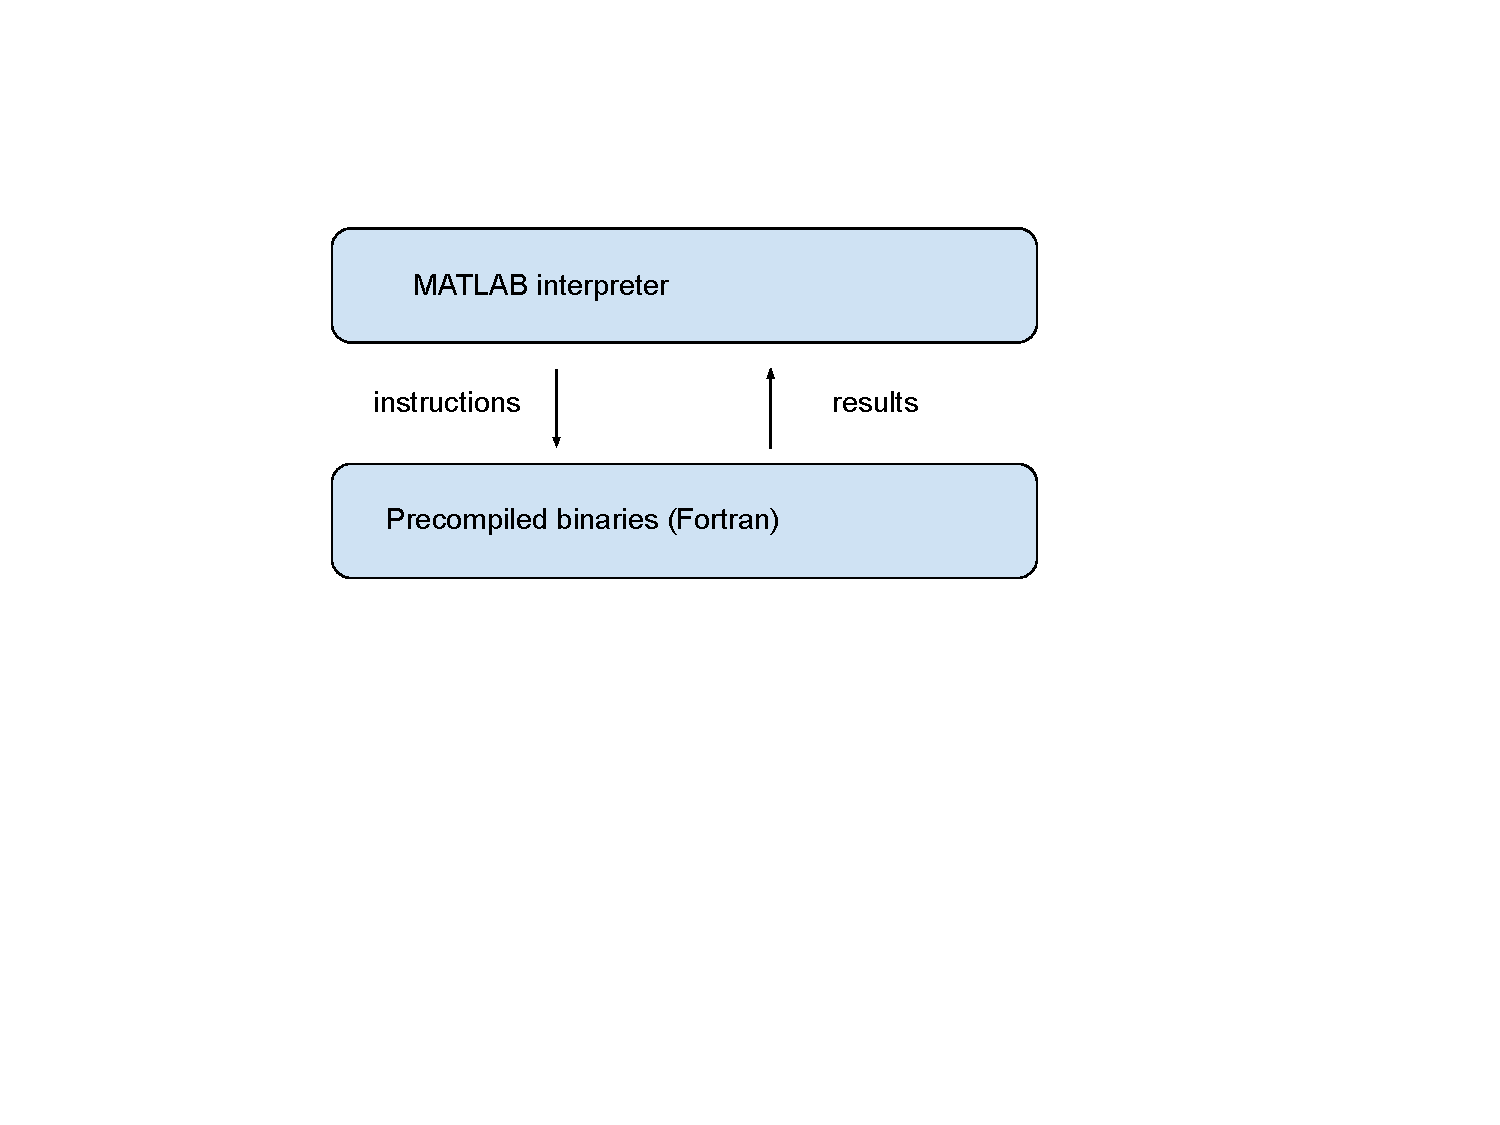
\includegraphics[trim={2cm 8cm 6cm 3cm},clip]{matlab.pdf}}
    \end{figure}


\end{frame}



\begin{frame}[fragile]
    
    \begin{minted}{matlab}
        A = [2.0, -1.0
             5.0, -0.5];

        b = [0.5, 1.0]';

        x = inv(A) * b
    \end{minted}
    
\end{frame}



    


\begin{frame}
    \frametitle{Python + NumPy}

    Open source MATLAB-like array operations within Python

    \begin{figure}
       \begin{center} % l b r t
        \scalebox{.6}{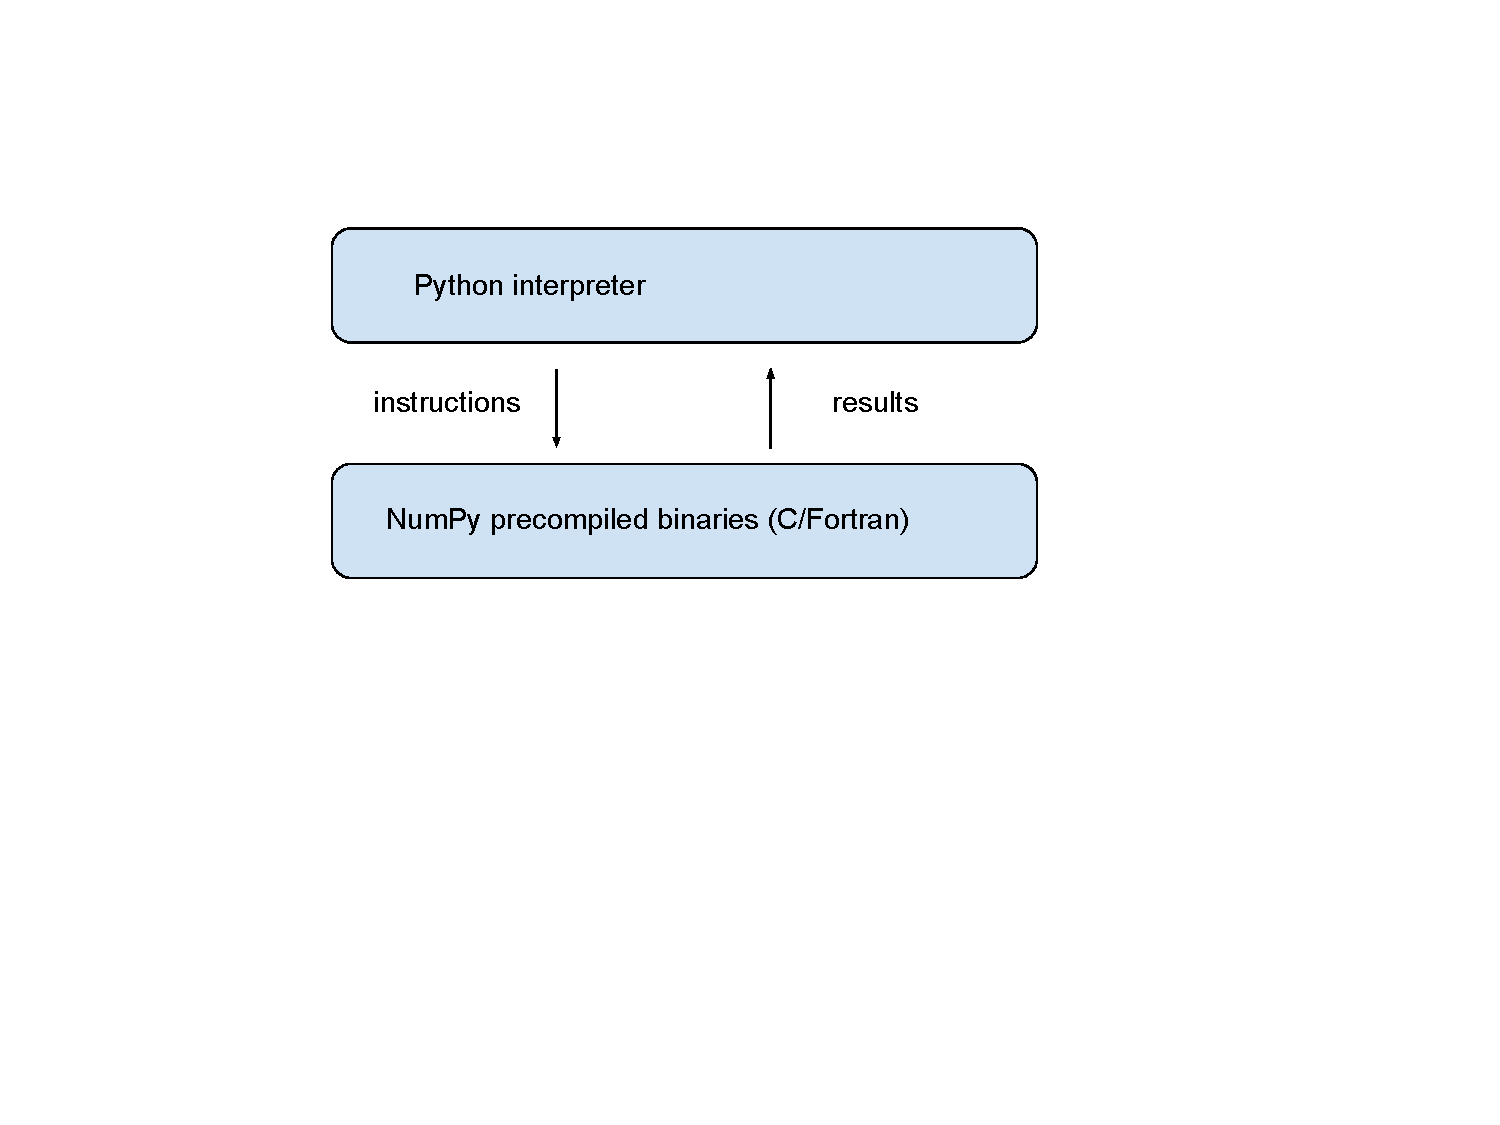
\includegraphics[trim={2cm 8cm 6cm 3cm},clip]{numpy.pdf}}
       \end{center}
    \end{figure}

\end{frame}

\begin{frame}[fragile]

    \begin{minted}{python}
        import numpy 

        A = ((2.0, -1.0),
             (5.0, -0.5))

        b = (0.5, 1.0)

        A, b = np.array(A), np.array(b)

        x = np.inv(A) @ b
    \end{minted}

\end{frame}

\begin{frame}
    
    \begin{enumerate}
        \item Arrays defined with high-level commands 
        \vspace{0.5em}
        %
        \begin{itemize}
            \item (Python / NumPy API)
        \end{itemize}
        %
        \vspace{0.5em}
        \item Execution takes place in an efficient low-level environment
        \vspace{0.5em}
        %
        \begin{itemize}
            \item Efficient machine code (compiled C / Fortran)
        \end{itemize}
        %
        \vspace{0.5em}
        \item Results are returned to the high-level interface
    \end{enumerate}

\end{frame}



\begin{frame}
    
    Advantages of NumPy / MATLAB

    \vspace{0.5em}
    \begin{itemize}
        \item Operations are passed to specialized machine code 
        \vspace{0.5em}
        \item Type-checking is \brown{paid per array, not per array element}
    \end{itemize}

    \vspace{0.5em}
    Disadvantages 

    \begin{itemize}
        \item Memory intensive (generates intermediate arrays)
        \vspace{0.5em}
        \item Limited --- how to accelerate the Solow code using NumPy?
        \vspace{0.5em}
        \item Specializes on \brown{types} but not on \brown{shapes}
    \end{itemize}


    \medskip
    The last point is important for modern hardware\ldots

\end{frame}


\begin{frame}[fragile]
    \frametitle{Julia --- rise of the JIT compilers}

    Can do MATLAB / NumPy style vectorized operations

    \begin{minted}{julia}
A = [2.0  -1.0
     5.0  -0.5]

b = [0.5  1.0]'

x = inv(A) * b
    \end{minted}
    

    \vspace{0.5em}
    \vspace{0.5em}
    But also has fast loops via an efficient JIT compiler

\end{frame}


\begin{frame}
    
    \Eg Suppose, again, that we want to compute 
    %
    \begin{equation*}
        k_{t+1} = s k_t^\alpha + (1 - \delta) k_t
    \end{equation*}
    %
    from some given $k_0$ 


    \vspace{0.5em}
    \vspace{0.5em}
    \vspace{0.5em}
    \vspace{0.5em}
    \begin{itemize}
        \item Iterative, not easily vectorized
    \end{itemize}

\end{frame}


\begin{frame}[fragile]
    
    \begin{minted}{julia}

function solow(k0, α=0.4, δ=0.1, n=1_000)
    k = k0
    for i in 1:(n-1)
        k = s * k^α + (1 - δ) * k
    end
    return k
end

solow(0.2)  # JIT-compiled at first call
    \end{minted}

    \vspace{0.5em}
    \vspace{0.5em}
    \vspace{0.5em}
    \vspace{0.5em}

    Julia accelerates \texttt{solow} at runtime via a JIT compiler

\end{frame}


\begin{frame}
    
    Pros:

    \begin{itemize}
        \item fast execution --- assuming correct type inference
        \vspace{0.2em}
        \item dynamically typed\ldots (but compiler wants type stability)
        \vspace{0.2em}
        \item elegant: close to the maths
    \end{itemize}

        \vspace{0.2em}
        \vspace{0.2em}
        \vspace{0.2em}
        \vspace{0.2em}
        \vspace{0.2em}
        \vspace{0.2em}
    Cons:

    \begin{itemize}
        \item Everything compiled might not be optimal 
        \vspace{0.2em}
        \begin{itemize}
            \item debugging is more challenging
            \vspace{0.2em}
            \item slow first runs
            \vspace{0.2em}
        \end{itemize}
        \vspace{0.2em}
        \item Repeated breaking changes and package instability
        \vspace{0.2em}
        \item Parallelization not well automated
    \end{itemize}

\end{frame}

\begin{frame}[fragile]
    \frametitle{Python + Numba --- same architecture, same speed}
    
    \begin{minted}{python}
from numba import jit

@jit(nopython=True)
def solow(k0, α=0.4, δ=0.1, n=1_000):
    k = k0
    for i in range(n-1):
        k = s * k**α + (1 - δ) * k
    return k

solow(0.2)
    \end{minted}


    Runs at same speed as Julia / C / Fortran

\end{frame}


\begin{frame}{New Paradigms}

    The technologies discussed above are all more than 10 years old
    
    \medskip
    Recently developed coding environments tend to be oriented towards AI

    \begin{itemize}
        \item PyTorch
            \medskip
        \item Google JAX
            \medskip
        \item Mojo, etc.
    \end{itemize}

    \medskip
    \medskip
    Sometimes these new environments are better\ldots and sometimes not

    \medskip
    We will discuss them later in the course

\end{frame}


\end{document}
